\section{Межмолекулярные взаимодействия. Водородная связь, ее природа, свойства и роль в жидкостях, молекулярных кристаллах и макромолекулах. Ван-дер-ваальсова связь, различные виды диполь-дипольных взаимодействий.}

\textbf{Межмолекулярное взаимодействие (ММВ)} --- взаимодействие молекул между собой, не приводящее к разрыву или образованию новых химических связей.\\

От ММВ зависят многие структурные, спектральные, термодинамические и др. свойства.\\

Существует несколько различных видов ММВ: большинство из них объединяются под названием \textbf{\textit{ван-дер-ваальсовых сил}}, имеющих универсальный характер (их наличие зависит от физических свойств), но существуют и спецефические виды, как \textbf{\textit{водородная связь}}, более близкая по свойствам к химической связи, но гораздо слабее её. Порядок величины таких взаимодействий --- 1--50 кДж/моль, т.е. гораздо меньше, чем хим. связей.\\

Причины возникновения сил Ван-дер-Ваальса - кулоновские силы взаимодействия между электронами и ядрами одной молекулы и ядрами и электронами другой. Силы Ван-дер-Ваальса зависят от расстояния между молекулами, их взаимной ориентации, строения, собственного дипольного момента и поляризуемости молекул. При больших межмолекулярных расстояниях (значительно больших, чем линейные размеры молекул) выделяют \textbf{три категории ММВ:}
\begin{itemize}
	\item \textbf{\textit{Электростатические (ориентационные)}} --- между полярными молекулами (диполь-диполь). 
	
	Возникают при такой взаимной ориентации молекул, что область локализации отрицательного заряда на одной молекуле и положительного на другой примерно совпадают, возникает притяжение. Например, \ce{HCl-HCl}.
	
	\item \textbf{\textit{Поляризационные (индукционные)}} --- между полярной и неполярной молекулами (постоянный диполь -- наведенный диполь).
	
	Под влиянием электростатического поля одной молекулы происходит деформация электронной оболочки другой молекулы, что приводит к понижению общей энергии = к притяжению. Пример: \ce{Br2-H2O}.
	
	\item \textbf{\textit{Дисперсионные}} --- между неполярными молекулами (наведенный диполь -- наведенный диполь).
	
	Определяется квантово-механическими флуктуациями электронной плотности частиц. Возникает корреляция движения электронов двух взаимодействующих молекул, среднее расстояние между ними несколько увеличивается, а энергия взаимодействия уменьшается. Данный вид взаимодействия реализуется между всеми частицами вне зависимости наличия у них заряда или собственных мультипольных моментов. Как пример: \ce{Cl2-Cl2}.
\end{itemize}

Притяжение тем больше, чем тяжелее молекула, больше её полярность или поляризуемость.\\

\textbf{Водородная связь} --- притяжение между атомом водорода (+) при полярной связи одной молекулы и атомом \ce{F, O, N} (–) при полярной связи другой молекулы.

\begin{figure}[H]
	\centering
	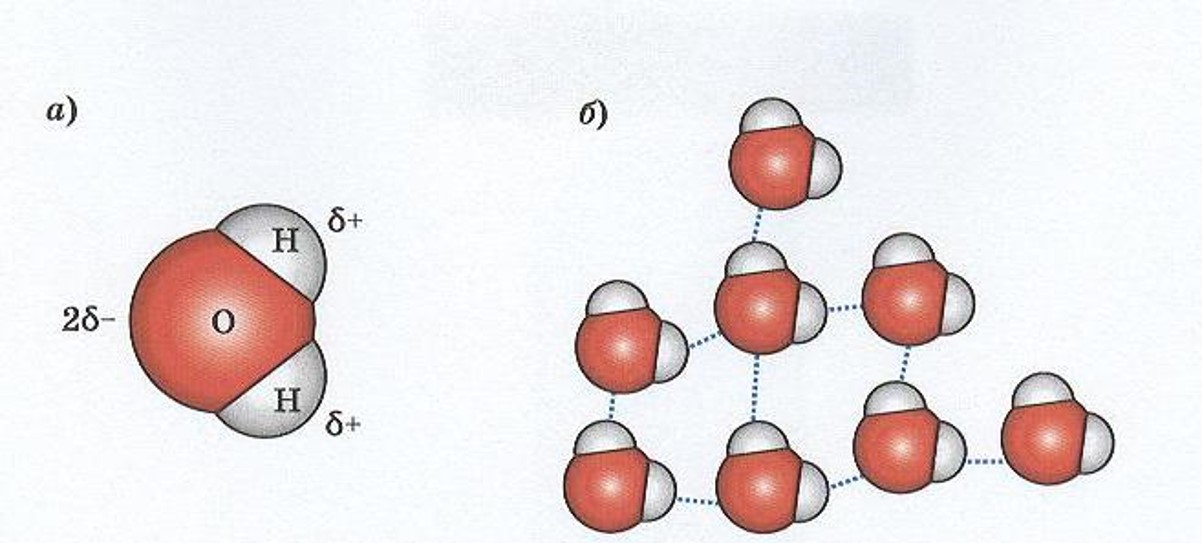
\includegraphics{Pictures/Vodorod.jpg}
	\caption{Водородные связи в воде.}
\end{figure}

Несмотря на то, что водород сильно связан с атомом в одной молекуле, он имеет небольшое, но заметное сродство к другому электроотрицательному атому. Такое взаимодействие обусловено малым размером поляризованного атома водорода (кроме валентного, электронов больше нет).\\

Водородная связь влияет на многие свойства вещества, такие как плотность, вязкость, поверхностное натяжение, кислотность, несмотря на то, что она сильно слабее химической связи.\\

Одним из доказательств наличия водородных связей является аномально высокая температура кипения бинарных соединений водорода с \textit{p}-элементами (см. картинку):

\begin{figure}[H]
	\centering
	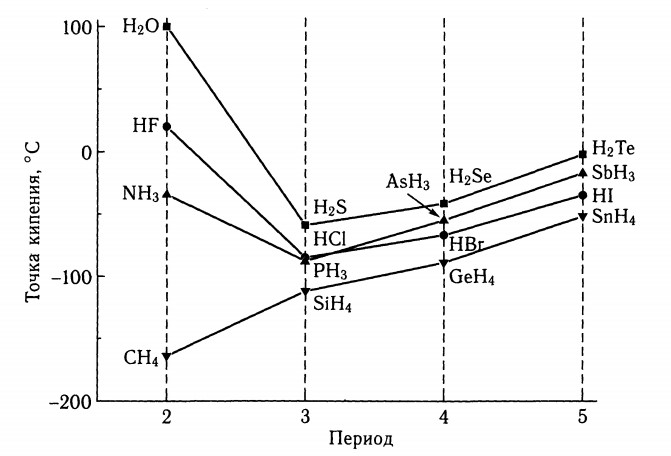
\includegraphics[width=0.7\linewidth]{Pictures/Temp.jpg}
	\caption{Нормальные температуры кипения соединений водорода с неметаллами.}
\end{figure}

Видно, что точки кипения для гидридов элементов \ce{F, O, N} сильно отклоняются от почти прямолинейной зависимости. Это легко объясняется наличием ММВ, вызванным сильными водородными связями.\\

Водородными связями легко объясняется каркасная структура льда, из-за чего он имеет меньшую плотность, чем вода.

\begin{figure}[H]
	\centering
	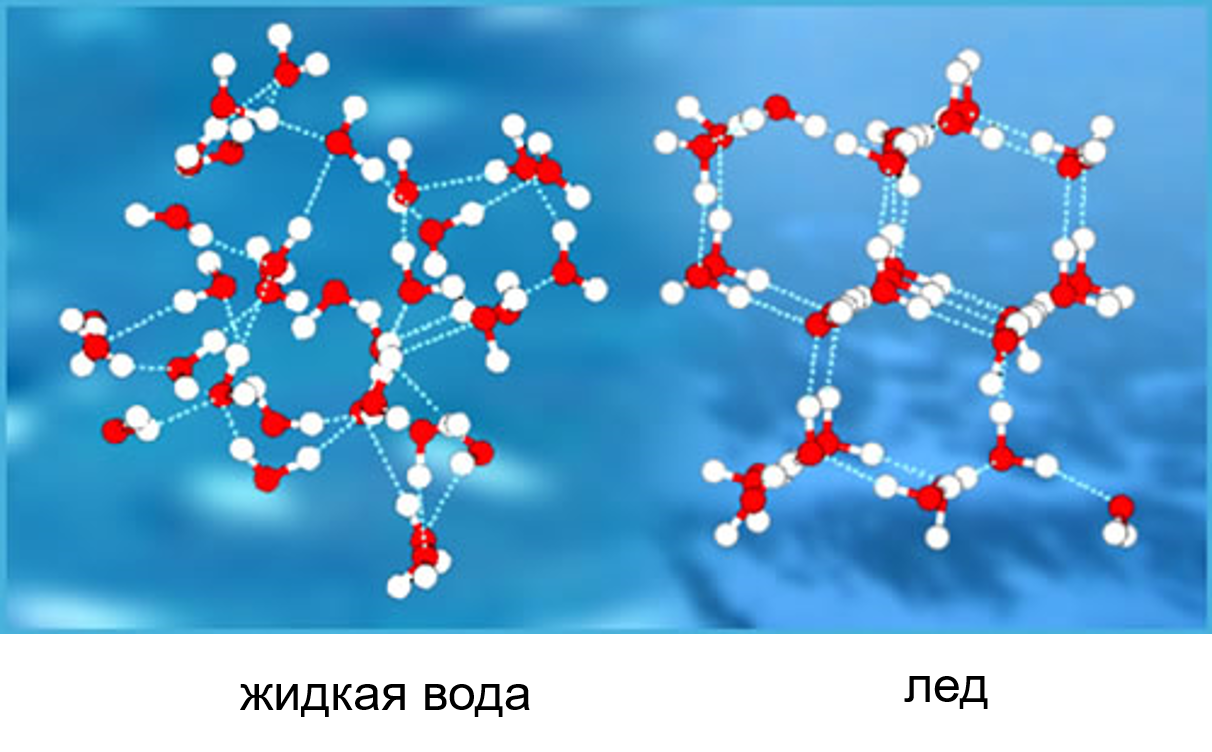
\includegraphics[width=0.7\linewidth]{Pictures/Led.png}
	\caption{Водородные связи в жидкой воде и льде.}
\end{figure}
